\documentclass[tikz]{standalone}
\usepackage{amsmath}
\definecolor{bg}{HTML}{171D2B}
\definecolor{aksen}{HTML}{F7B538}
\definecolor{teks}{HTML}{FFFFFF}
\pagecolor{bg}
\begin{document}
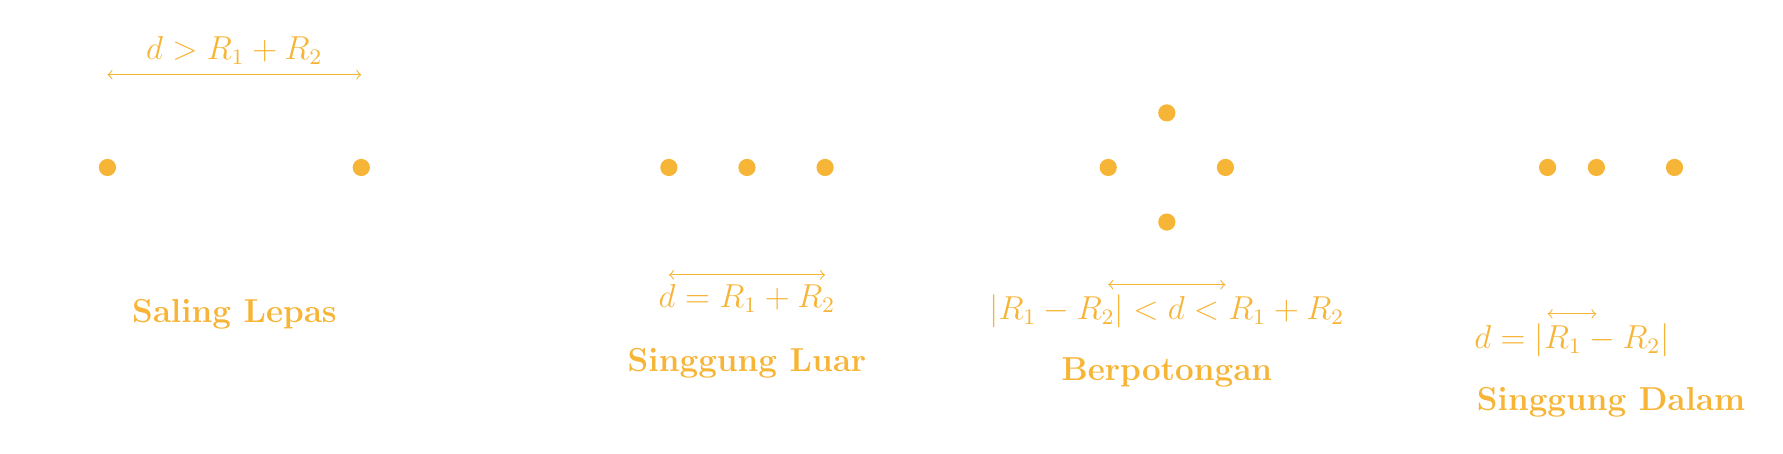
\begin{tikzpicture}[scale=0.62,
  ling/.style={draw=teks,very thick},
  titik/.style={circle,fill=aksen,inner sep=2.2pt},
  lab/.style={text=teks,font=\large},
  sub/.style={text=aksen,font=\large\bfseries}]
% (a) saling lepas
\begin{scope}[shift={(0,0)}]
  \draw[ling] (0,0) circle (1.6);
  \draw[ling] (5.2,0) circle (1.6);
  \node[titik] at (0,0) {}; \node[titik] at (5.2,0) {};
  \node[lab,below=4pt] at (0,0) {$P_1$};
  \node[lab,below=4pt] at (5.2,0) {$P_2$};
  \draw[aksen,<->] (0,1.9) -- (5.2,1.9);
  \node[sub,above] at (2.6,1.9) {$d>R_1+R_2$};
  \node[sub] at (2.6,-3.0) {Saling Lepas};
\end{scope}
% (b) bersinggungan luar
\begin{scope}[shift={(11.5,0)}]
  \draw[ling] (0,0) circle (1.6);
  \draw[ling] (3.2,0) circle (1.6);
  \node[titik] at (0,0) {}; \node[titik] at (3.2,0) {};
  \node[titik] at (1.6,0) {};
  \node[lab,below=4pt] at (0,0) {$P_1$};
  \node[lab,below=4pt] at (3.2,0) {$P_2$};
  \node[lab,above=4pt] at (1.6,0) {$A$};
  \draw[aksen,<->] (0,-2.2) -- (3.2,-2.2);
  \node[sub,below] at (1.6,-2.2) {$d=R_1+R_2$};
  \node[sub] at (1.6,-4.0) {Singgung Luar};
\end{scope}
% (c) berpotongan
\begin{scope}[shift={(20.5,0)}]
  \draw[ling] (0,0) circle (1.6);
  \draw[ling] (2.4,0) circle (1.6);
  \node[titik] at (0,0) {}; \node[titik] at (2.4,0) {};
  \coordinate (A1) at (1.2,1.118);
  \coordinate (A2) at (1.2,-1.118);
  \node[titik] at (A1) {}; \node[titik] at (A2) {};
  \node[lab,below=4pt] at (0,0) {$P_1$};
  \node[lab,below=4pt] at (2.4,0) {$P_2$};
  \node[lab,right=3pt] at (A1) {$A$};
  \node[lab,right=3pt] at (A2) {$B$};
  \draw[aksen,<->] (0,-2.4) -- (2.4,-2.4);
  \node[sub,below] at (1.2,-2.4) {$|R_1-R_2|<d<R_1+R_2$};
  \node[sub] at (1.2,-4.2) {Berpotongan};
\end{scope}
% (d) singgung dalam
\begin{scope}[shift={(29.5,0)}]
  \draw[ling] (0,0) circle (2.6);
  \draw[ling] (1.0,0) circle (1.6);
  \node[titik] at (0,0) {}; \node[titik] at (1.0,0) {};
  \node[titik] at (2.6,0) {};
  \node[lab,below=4pt] at (0,0) {$P_1$};
  \node[lab,above=4pt] at (1.0,0) {$P_2$};
  \node[lab,above right=2pt] at (2.6,0) {$A$};
  \draw[aksen,<->] (0,-3.0) -- (1.0,-3.0);
  \node[sub,below] at (0.5,-3.0) {$d=|R_1-R_2|$};
  \node[sub] at (1.3,-4.8) {Singgung Dalam};
\end{scope}
\end{tikzpicture}
\end{document}